% Autor: Leonhard Segger, Alexander Neuwirth
% Datum: 2017-10-30
\documentclass[
	% Papierformat
	a4paper,
	% Schriftgröße (beliebige Größen mit „fontsize=Xpt“)
	12pt,
	% Schreibt die Papiergröße korrekt ins Ausgabedokument
	pagesize,
	% Sprache für z.B. Babel
	ngerman
]{scrartcl}

% Achtung: Die Reihenfolge der Pakete kann (leider) wichtig sein!
% Insbesondere sollten (so wie hier) babel, fontenc und inputenc (in dieser
% Reihenfolge) als Erstes und hyperref und cleveref (Reihenfolge auch hier
% beachten) als Letztes geladen werden!

% Silbentrennung etc.; Sprache wird durch Option bei \documentclass festgelegt
\usepackage{babel}
% Verwendung der Zeichentabelle T1 (Sonderzeichen etc.)
\usepackage[T1]{fontenc}
% Legt die Zeichenkodierung der Eingabedatei fest, z.B. UTF-8
\usepackage[utf8]{inputenc}
% Schriftart
\usepackage{lmodern}
% Zusätzliche Sonderzeichen
\usepackage{textcomp}

% Mathepaket (intlimits: Grenzen über/unter Integralzeichen)
\usepackage[intlimits]{amsmath}
% Ermöglicht die Nutzung von \SI{Zahl}{Einheit} u.a.
\usepackage{siunitx}
% Zum flexiblen Einbinden von Grafiken (\includegraphics)
\usepackage{graphicx}
% Abbildungen im Fließtext
\usepackage{wrapfig}
% Abbildungen nebeneinander (subfigure, subtable)
\usepackage{subcaption}
% Funktionen für Anführungszeichen
\usepackage{csquotes}
% Zitieren, Bibliographie
\usepackage{biblatex}


% Zur Darstellung von Webadressen
\usepackage{url}
%chemische Formeln
\usepackage[version=4]{mhchem}
% siunitx: Deutsche Ausgabe, Messfehler getrennt mit ± ausgeben
\usepackage{floatrow}
\floatsetup[table]{capposition=top}
\usepackage{float}
% Verlinkt Textstellen im PDF-Dokument
\usepackage[unicode]{hyperref}
% "Schlaue" Referenzen (nach hyperref laden!)
\usepackage{cleveref}
\sisetup{
	locale=DE,
	separate-uncertainty
}
\bibliography{14Mo_A2_30-04-2018_References}

\begin{document}
	
	\begin{titlepage}
		\centering
		{\scshape\LARGE Versuchsbericht zu \par}
		\vspace{1cm}
		{\scshape\huge A2 - Franck-Hertz-Versuch \par} 
		\vspace{2.5cm}
		{\LARGE Gruppe 14Mo \par}
		\vspace{0.5cm}
		
		{\large Alexander Neuwirth (E-Mail: a\_neuw01@wwu.de) \par}
		{\large Leonhard Segger (E-Mail: l\_segg03@uni-muenster.de) \par}
		\vfill
		
		durchgeführt am 30.04.2018\par
		betreut von\par
		{\large Fabian Schöttke}
		
		\vfill
		
		{\large \today\par}
	\end{titlepage}
	\tableofcontents
	\newpage

	%TODO mehr TODO in Default	

	\section{Kurzfassung}
	%TODO Hypothese	und deren Ergebnis
	%TODO Ergebnisse, auch Zahlen, mindestens wenn's halbwegs Sinn ergibt
	%TODO Was wurde gemacht
	
	\section{Methoden}
	%TODO Bilder von der Website klauen
	Untersucht wurde eine Franck-Hertz-Röhre mit Quecksilberfüllung und eine mit Neonfüllung.
	Diese wurden, wie in  \cref{Roehren_Schaltung} dargestellt, verschaltet. %ist das schön?
	Die Quecksilberröhre befand sich in einem Ofen, der sie auf bis zu \SI{300}{\degreeCelsius} aufheizen kann.
	Der Anodenstrom ist sehr klein, weshalb er vom Betriebsgerät in eine Spannung $U_A$ umgewandelt wurde, die zum Anodenstrom proportional ist.
	
	Zunächst wurde die $I_A/U_B$-Charakteristik der Röhre mit Quecksilberfüllung bei Zimmertemperatur aufgenommen.
	Dazu wurde die Beschleunigungsspannung $U_B$ langsam erhöht und diese sowie die Spannung $U_A$ gemessen.
	
	Im Anschluss wurde der Ofen auf ca. \SI{180}{\degreeCelsius} erhitzt.
	Dann wurde das Betriebsgerät so eingestellt, dass es eine Dreieckspannung mit einer Frequenz von \SI{60}{\hertz} als Beschleunigungsspannung ausgibt.
	Der resultierende Anodenstrom wurde zunächst mit einem Oszilloskop betrachtet und Bremsspannung $U_B$ und Heizstrom $I_H$ so eingestellt, dass sich mindestens drei Minima der Franck-Hertz-Kurve ablesen ließen.
	Dann wurde mithilfe manueller Reglung der Beschleunigungsspannung die $I_A/U_B$-Charakteristik wie zuvor aufgenommen und die Temperatur im Ofen gemessen.
	
	Analog wurde die Neon-Röhre bei Raumtemperatur untersucht, wobei hier zusätzlich ein Steuergitter (mit Spannung $U_S$) verwendet wurde, um störende Einflüsse durch Abstoßung der Elektronen untereinander zu verringern. %TODO Ist das so korrekt?
	
	\begin{figure}[H]
		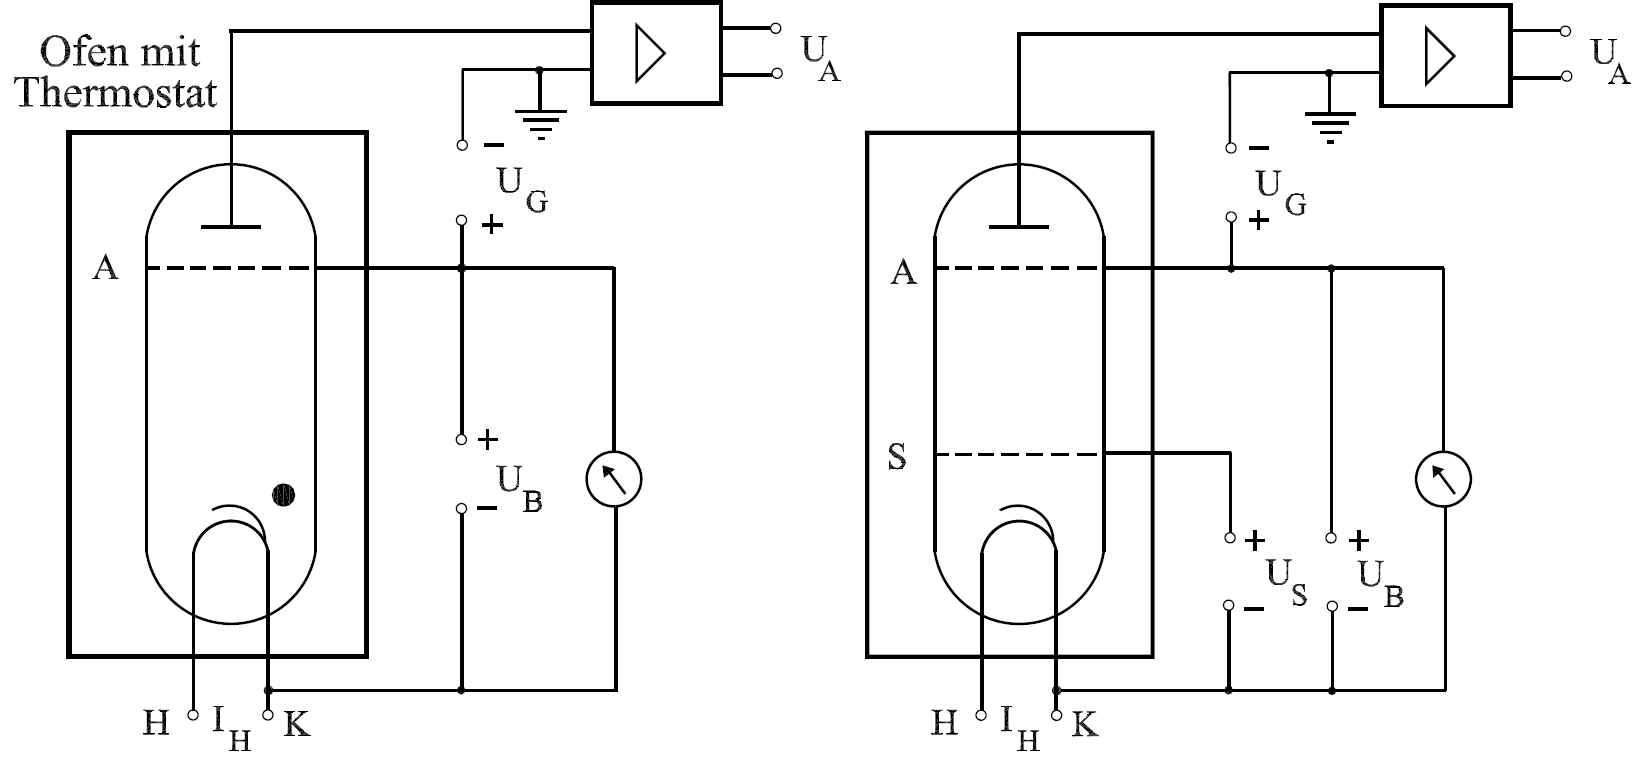
\includegraphics[width=0.7\textwidth]{Roehren}
		\centering
		\caption{Schaltungen der Franck-Hertz-Röhren mit Quecksilber (links) und Neon (rechts).\cite{Roehren} }
		\label{Roehren_Schaltung}
		\centering
	\end{figure}

	\section{Ergebnisse und Diskussion}
	%TODO Datenanalyse -> Überschrift?
	%TODO Unsicherheiten
	

	\subsection{Beobachtung}

	\subsection{Diskussion}
	%TODO Bezug/Nutzten oder sonst was
	%TODO auch hier die Hypothese wiederholen
	
	\section{Schlussfolgerung}
	%TODO Rückgriff auf Hypothese und drittes Nennen dieser
	
	%TODO Quellen zitieren, Websiten mit Zugriffsdatum
	%TODO Verweise auf das Laborbuch (sind erlaubt)
	%TODO Tabelle + Bilder mit Beschriftung
	\printbibliography
\end{document}
